\chapter{Rectificador Controlado de Silicio}
  \begin{wrapfigure}{R}{0.3\textwidth}
  \vspace{-1cm}
    \centering
    \resizebox{!}{\linewidth}{
    \begin{tikzpicture}
	\begin{pgfonlayer}{nodelayer}
		\node [style=none] (0) at (-1, 2) {};
		\node [style=none] (1) at (1, 2) {};
		\node [style=none] (2) at (-1, 1) {};
		\node [style=none] (3) at (1, 1) {};
		\node [style=none] (4) at (-1, 0) {};
		\node [style=none] (5) at (1, 0) {};
		\node [style=none] (6) at (-1, -1) {};
		\node [style=none] (7) at (1, -1) {};
		\node [style=none] (8) at (-1, -2) {};
		\node [style=none] (9) at (1, -2) {};
		\node [style=none] (10) at (-0.5, -2) {};
		\node [style=none] (11) at (0.5, -2) {};
		\node [style=none] (12) at (-0.5, -2.25) {};
		\node [style=none] (13) at (0.5, -2.25) {};
		\node [style=none] (14) at (-0.5, 2.25) {};
		\node [style=none] (15) at (0.5, 2.25) {};
		\node [style=none] (16) at (-0.5, 2) {};
		\node [style=none] (17) at (0.5, 2) {};
		\node [style=none] (18) at (-1.25, -0.25) {};
		\node [style=none] (19) at (-1, -0.25) {};
		\node [style=none] (20) at (-1.25, -0.75) {};
		\node [style=none] (21) at (-1, -0.75) {};
		\node [style=none] (22) at (-1.25, -0.5) {};
		\node [style=none] (23) at (0, -2.25) {};
		\node [style=none] (24) at (0, 2.25) {};
		\node [style=none] (25) at (0, 3) {};
		\node [style=none] (26) at (-2, -0.5) {};
		\node [style=none] (27) at (0, -3) {};
		\node [style=none] (28) at (0, 1.5) {p};
		\node [style=none] (29) at (0, 0.5) {n};
		\node [style=none] (30) at (0, -0.5) {p};
		\node [style=none] (31) at (0, -1.5) {n};
		\node [style=none] (32) at (0, -3.25) {K};
		\node [style=none] (33) at (0, 3.25) {A};
		\node [style=none] (34) at (-2.25, -0.5) {G};
	\end{pgfonlayer}
	\begin{pgfonlayer}{edgelayer}
		\draw [style=fill2] (3.center)
			 to (2.center)
			 to (0.center)
			 to (1.center)
			 to cycle;
		\draw [style=fill2] (4.center)
			 to (6.center)
			 to (7.center)
			 to (5.center)
			 to cycle;
		\draw [style=fill3] (4.center)
			 to (5.center)
			 to (3.center)
			 to (2.center)
			 to cycle;
		\draw [style=fill3] (8.center)
			 to (9.center)
			 to (7.center)
			 to (6.center)
			 to cycle;
		\draw [style=fill4] (10.center)
			 to (12.center)
			 to (13.center)
			 to (11.center)
			 to cycle;
		\draw [style=fill4] (14.center)
			 to (16.center)
			 to (17.center)
			 to (15.center)
			 to cycle;
		\draw [style=fill4] (18.center)
			 to (20.center)
			 to (21.center)
			 to (19.center)
			 to cycle;
		\draw (22.center) to (26.center);
		\draw (24.center) to (25.center);
		\draw (23.center) to (27.center);
	\end{pgfonlayer}
\end{tikzpicture}

    }
    \caption{estructura interna del SCR.}
    \label{fig:scr_si}
  \end{wrapfigure}
  Un SCR (rectificador controlado de silicio, silicon-controlled rectifier) es un dispositivo pnpn de 4 capas similar al
  diodo de 4 capas pero con tres terminales: ánodo, cátodo y compuerta. En la figura \ref{fig:scr_si} puede ver la
  construccion basica del mismo, y su simbolo esquematico.

  \section{Activación del SCR}
    Cuando la corriente en la compuerta, $I_G$, es cero, por lo que el dispositivo actúa como un diodo de 4 capas en el
    estado de apagado. En este estado, la muy alta resistencia entre el ánodo y el cátodo pueden ser simulados de forma
    aproximada por un interruptor abierto. Cuando se aplica un pulso (disparo) positivo de corriente a la compuerta, el
    dispositivo se enciende, generando un camino de baja resistencia para permitir el flujo de corriente entre anodo y
    catodo. El SCR se puede activar tambien por voltake entre anodo y catodo, ya que mientras que $I_G = 0$, el componente
    se comportara como un diodo de 4 capas.

    Se propuso analizar las regiones de acrivacion y corrientes de codo del SCR seleccionado y compararlas con las
    provistas por el fabricante en el datasheet. Para nuestra practica, seleccionamos el TYN612M. Para analizar las
    diferentes regiones, se realizaran 3 pruebas:
    \begin{itemize}
      \item Curva de $I_G = f_{(V_G)}$ para $V_{AK} = 0V$,
      \item Curva de $I_A = f_{(V_{AK})}$ para $V_G = 0V$,
      \item Curva de $I_A = f_{(V_G)}$ para $V_{AK} = 100V$.
    \end{itemize}

    Por cuestiones de seguridad, la curva de $I_A = f_{(V_{AK})}$ para $V_G = 0V$ solo se realizara en simulacion.

    \subsection{Curva $I_G = f_{(V_G)}$}
      Para lograr esta curva, la unica condicion que se debe aplicar es mantener $V_{AK} = 0V$ en todo momento,
      mientras se varia el $V_G$.

      \subsubsection{Actividad de simulacion}
        Se propuso realizar un barrido lineal de la tension $V_G$ mientras que $V_{AK} = 0V$. El barrido es de $0V$ a
        $20V$ en pasos de $100mV$. Para trazar esta curva, el circuito utilizado es el de la figura \ref{crkt:scr_vak0}
        y los parametros de simulacion se pueden ver en \ref{list:scr_vak0}.
        \begin{figure}[!ht]
          \centering
          \begin{minipage}{0.45\textwidth}
            \centering
            \begin{tikzpicture}
	% Paths, nodes and wires:
	\draw (0, 2.3) to[american voltage source, l={$V_1$}] (0, -0);
	\draw (6.77, 4.5) to[american voltage source, l={$V_2$}] (6.77, 2.5);
	\draw (0, 2.3) to[american resistor, l={$4K7$}] (3, 2.3);
	\draw (3.77, 4) to[american resistor, l={$4K7$}] (3.77, 7);
	\draw (3.77, 4) to[empty thyristor, mirror] (3.77, 2);
	\draw (6.77, 4.5) -- (6.77, 7) -- (3.77, 7);
	\draw (3.77, 2) -| (3.77, -0) -- (6.77, -0) -| (6.77, 2.5);
	\draw (0, -0) -- (0.02, -0) -- (3.77, -0);
	\draw (3, 2.3) to[qvprobe, l_={$V_G$}] (3, -0);
\end{tikzpicture}
            \caption{circuito del SCR a simular}
            \label{crkt:scr_vak0}
          \end{minipage}
          \hfill
          \begin{minipage}{0.45\textwidth}
            \centering
          \begin{lstlisting}[style=ltspice, caption={Parámetros de simulación LTspice}, label=list:scr_vak0]
.dc V1 0 20 100m
          \end{lstlisting}
          \end{minipage}
        \end{figure}

      Revise la seccion \ref{annex:scr_model} para ver el modelo SPICE utilzado para las simulaciones.
      \begin{figure}[!ht]
        \begin{tikzpicture}
          \begin{axis}[
            width=14cm,
            height=5.5cm,
            xlabel={$V_G$ [mV]},
            ylabel={$I_G$ [mA]},
            grid=both,
            minor tick num=1,
            scale only axis,
            enlargelimits=false,
              title={$I_G = f_{(V_G)}$},
            extra x ticks={300},
            extra x tick style={
              grid style={red, thick, dashed},
              tick style={red},
              tick label style={red}
             },
            scaled ticks=false,
            restrict x to domain=0:400,
            xmin=0, xmax=400
          ]
          \addplot[
            color=blue,
            mark=none,
            thick,
          ] table[
            col sep=tab,
            header=true,
            x expr=\thisrow{V(vg)}*1000,
            y expr=\thisrow{Ix(U1:G)}*1000
          ] {simulations/ig_vg_vak0.txt};
          \end{axis}
        \end{tikzpicture}
          \caption{grafica de la corriente de gate en funcion de la tension de gate.}
          \label{graph:scr_ig_vg_vak0}
      \end{figure}

      La curva relevada se puede ver en la figura \ref{graph:scr_ig_vg_vak0}, y esta es bastante similar a la curva de
      un diodo, con el cambio de que el potencial en el que empieza a conducir es menor. Esto se debe a que la union
      presente entre gate y catodo es, a los ojos del circuito de gate, un simple diodo.

      \subsubsection{Actividad de Laboratorio}
        Para esta actividad, en vez de variar la fuente, esta se mantuvo fija, y usando un potenciometro fuimos variando
        su resistencia, provocando un cambio en la $V_G$ y la $I_G$. El circuito utilizado se puede ver en la figura
        \ref{crkt:scr_vak0_lab}.

        \begin{figure}[!ht]
          \centering
          \begin{minipage}{0.7\textwidth}
            \centering
            \resizebox{1\textwidth}{!}{
            \begin{tikzpicture}
	% Paths, nodes and wires:
	\draw (0.56, 2.3) to[american resistor, l={$4K7$}] (3.56, 2.3);
	\draw (7.83, 4) to[american resistor, l={$4K7$}] (7.83, 7);
	\draw (7.83, 4) to[empty thyristor, mirror] (7.83, 2);
	\draw (3.56, 2.3) to[qiprobe, l={$I_G$}] (5.56, 2.3);
	\draw (3.56, 2.3) to[qvprobe, l={$V_G$}] (3.56, -0);
	\draw (7.83, 2) to[qiprobe, l={$I_A$}] (7.83, -0);
	\draw (5.56, 2.3) to[normal open switch, l={$SW_1$}] (7.06, 2.3);
	\draw (10.06, 4) to[qvprobe, l_={$V_{AK}$}] (10.06, -0);
	\draw (11.06, 7) to[qvprobe, l={$V_i$}] (11.06, -0);
	\draw (0, 3.925) to[american potentiometer, l_={$5K$}] (0, 0.675);
	\draw (0, 0.675) |- (3.56, -0);
	\draw (3.56, -0) -- (7.83, -0) -- (10.06, -0) -- (11.06, -0);
	\node[vcc](N1) at (0, 7){} node[anchor=south] at (N1.text){$+20V$};
	\node[vcc](N2) at (7.83, 7){} node[anchor=south] at (N2.text){$V_i$};
	\draw (11.06, 7) |- (7.83, 7);
	\draw (10.06, 4) |- (7.83, 4);
	\draw (0, 7) -- (0, 3.925);
	\node[ground] at (7.83, -0){};
\end{tikzpicture}
            }
            \caption{circuito a implementar en el laboratorio.}
            \label{crkt:scr_vak0_lab}
          \end{minipage}
          \hfill
          \begin{minipage}{0.25\textwidth}
            \centering
            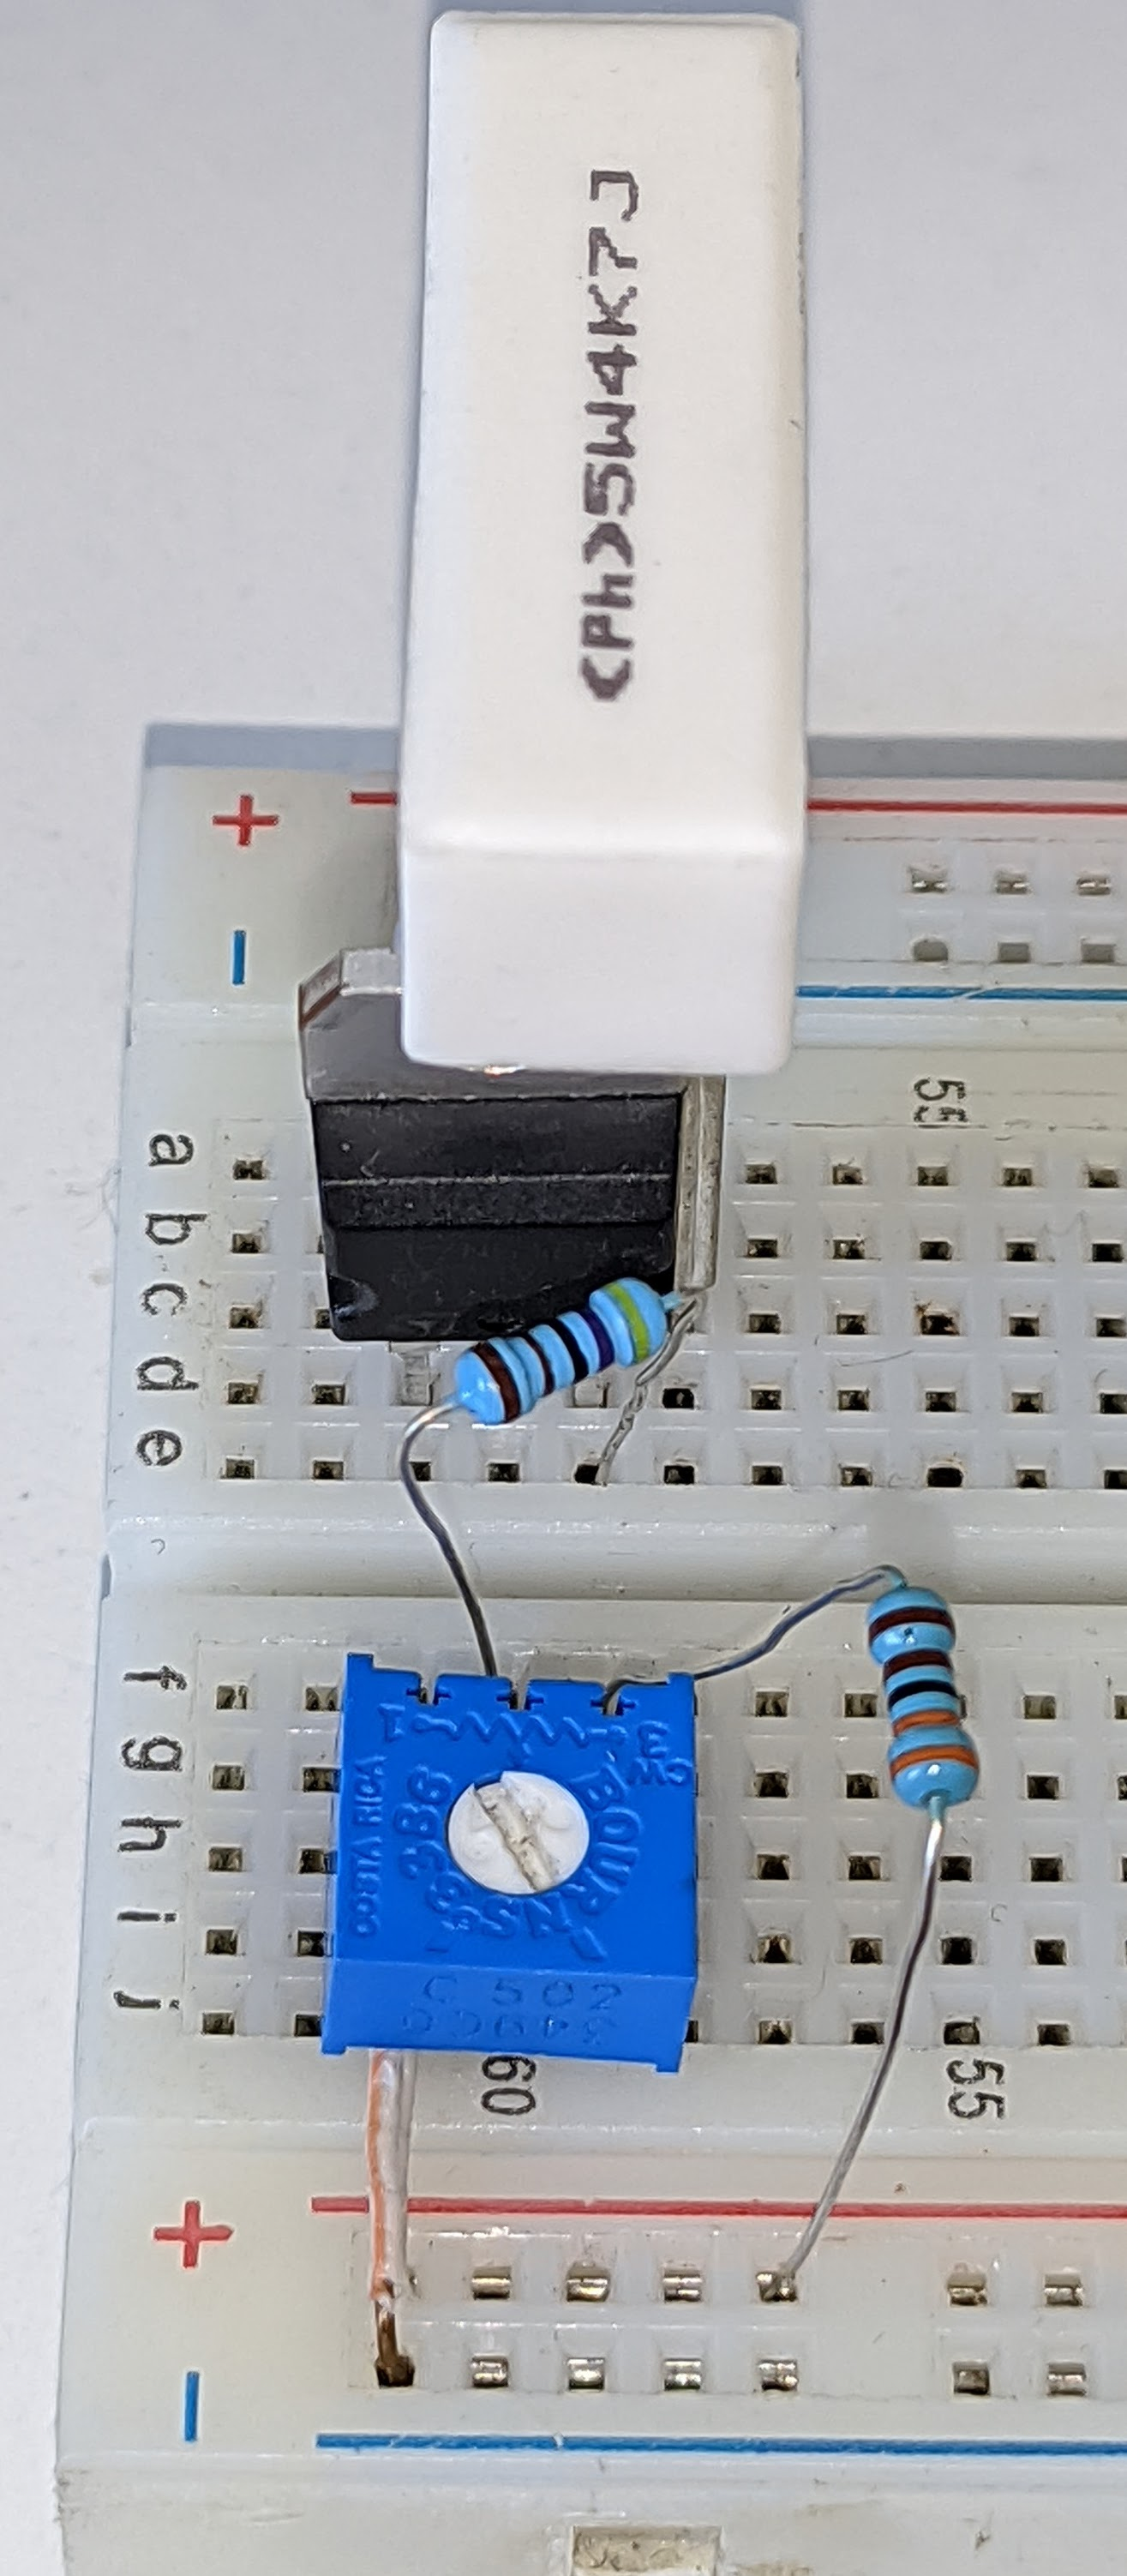
\includegraphics[width=0.8\textwidth]{pictures/prot_scr.jpg}
            \caption{circuito implementado en el laboratorio.}
          \end{minipage}
        \end{figure}

        Los datos relevados en el laboratorio se pueden ver en la tabla \ref{tab:scr_vak0_lab} y en la figura
        \ref{graph:scr_ig_vg_vak0_lab}. La curva es muy similar a la del diodo, solo que con un potencial de
        conduccion mas bajo que el diodo comun de silicio.

        \begin{figure}[!ht]
          \centering
          \begin{minipage}{0.3\textwidth}
            \centering
            \begin{tabular}{c|c}
              $V_G$ & $I_G$ \\ \hline
              0     & 0     \\
            \end{tabular}
            \caption{datos relvados en el laboratorio}
            \label{tab:scr_vak0_lab}
          \end{minipage}
          \hfill
          \begin{minipage}{0.6\textwidth}
            \begin{tikzpicture}
              \begin{axis}[
                width=8cm,
                height=5.5cm,
                xlabel={$V_G$ [mV]},
                ylabel={$I_G$ [mA]},
                grid=both,
                minor tick num=1,
                scale only axis,
                enlargelimits=false,
                  title={$I_G = f_{(V_G)}$},
                extra x ticks={300},
                extra x tick style={
                  grid style={red, thick, dashed},
                  tick style={red},
                  tick label style={red}
                 },
                scaled ticks=false,
                restrict x to domain=0:400,
                xmin=0, xmax=400
              ]
              \addplot[
                color=blue,
                mark=none,
                thick,
              ] table[
                col sep=tab,
                header=true,
                x expr=\thisrow{V(vg)}*1000,
                y expr=\thisrow{Ix(U1:G)}*1000
              ] {simulations/ig_vg_vak0.txt};
              \end{axis}
            \end{tikzpicture}
            \caption{grafica $I_G = f_{(V_G)}$ relevada en el laboratorio.}
            \label{graph:scr_ig_vg_vak0_lab}

          \end{minipage}
        \end{figure}

      \subsection{Curva $I_A = f_{(V_{AK})}$}
        Para lograr esta curva, la unica condicion que se debe aplicar es mantener $V_G = 0V$ en todo momento,
        mientras se varia el $V_{AK}$.
          Se propuso realizar un barrido lineal de la tension $V_{AK}$ mientras que $V_G = 0V$. El barrido es de $0V$ a
          $800V$ en pasos de $10V$. Para trazar esta curva, el circuito utilizado es el de la figura \ref{crkt:scr_vg0}
          y los parametros de simulacion se pueden ver en \ref{list:scr_vg0}.
          \begin{figure}[!ht]
            \centering
            \begin{minipage}{0.45\textwidth}
              \centering
              \begin{tikzpicture}
	% Paths, nodes and wires:
	\draw (0, 2.3) to[american voltage source, l={$V_1$}] (0, -0);
	\draw (6.77, 4.5) to[american voltage source, l={$V_2$}] (6.77, 2.5);
	\draw (0, 2.3) to[american resistor, l={$4K7$}] (3, 2.3);
	\draw (3.77, 4) to[american resistor, l={$4K7$}] (3.77, 7);
	\draw (3.77, 4) to[empty thyristor, mirror] (3.77, 2);
	\draw (6.77, 4.5) -- (6.77, 7) -- (3.77, 7);
	\draw (3.77, 2) -| (3.77, -0) -- (6.77, -0) -| (6.77, 2.5);
	\draw (0, -0) -- (0.02, -0) -- (3.77, -0);
	\draw (5.25, 4) to[qvprobe, l={$V_{AK}$}] (5.25, -0);
	\draw (5.25, 4) |- (3.77, 4);
\end{tikzpicture}
              \caption{circuito del SCR a simular}
              \label{crkt:scr_vg0}
            \end{minipage}
            \hfill
            \begin{minipage}{0.45\textwidth}
              \centering
            \begin{lstlisting}[style=ltspice, caption={Parámetros de simulación LTspice}, label=list:scr_vg0]
.dc V2 0 800 10
            \end{lstlisting}
            \end{minipage}
          \end{figure}

          \begin{figure}[!ht]
            \begin{tikzpicture}
              \begin{axis}[
                width=14cm,
                height=5.5cm,
                xlabel={$V_{AK}$ [V]},
                ylabel={$I_{AK}$ [mA]},
                grid=both,
                minor tick num=1,
                scale only axis,
                enlargelimits=false,
                  title={$I_{AK} = f_{(V_{AK})}$},
                extra x tick style={
                  grid style={red, thick, dashed},
                  tick style={red},
                  tick label style={red}
                 },
                extra y tick style={
                  grid style={red, thick, dashed},
                  tick style={red},
                  tick label style={red}
                 },
                scaled ticks=false,
                restrict x to domain=0:3,
                xmin=0, xmax=3
              ]
              \addplot[
                color=blue,
                mark=none,
                thick,
              ] table[
                col sep=tab,
                header=true,
                x expr=\thisrow{V(va)},
                y expr=\thisrow{Ix(U1:A)}*1000
              ] {simulations/iak_vak_vg0.txt};
              \end{axis}
            \end{tikzpicture}
              \caption{grafica de la corriente de anodo en funcion de la tension anodo-catodo.}
              \label{graph:scr_iak_vak_vg0}
          \end{figure}

          Como se puede ver en la figura \ref{graph:scr_iak_vak_vg0}, la curva obtenida no se parece a la curva
          caracteristica de los SCR. De hecho parece la curva de tension corriente de una resistencia. Esto se puede
          deber a que el modelo SPICE no tiene ese comportamiento tenido en cuenta. No encontramos otro modelo que si lo
          tuviese, por lo que no pudimos incluir la grafica correcta.

    \subsection{Curva $I_A = f_{(V_G)}$}
      Para esta curva, se fijara $V_{AK} = 100V$ y haciendo un barrido lineal de $V_G$ trazaremos la curva y
      encontraremos el punto donde el SCR se dispara por corriente de gate.

      \subsubsection{Actividad de Simulacion}
        Se propuso realizar un barrido lineal de la tension $V_g$ mientras que $V_{AK} = 100V$. El barrido es de $0V$ a
        $20V$ en pasos de $100mV$. Para trazar esta curva, el circuito utilizado es el de la figura \ref{crkt:scr_vak100}
        y los parametros de simulacion se pueden ver en \ref{list:scr_vak100}.
        \begin{figure}[!ht]
          \centering
          \begin{minipage}{0.45\textwidth}
            \centering
            \begin{tikzpicture}
	% Paths, nodes and wires:
	\draw (0, 2.3) to[american voltage source, l={$V_1$}] (0, -0);
	\draw (6.77, 4.5) to[american voltage source, l={$V_2$}] (6.77, 2.5);
	\draw (0, 2.3) to[american resistor, l={$4K7$}] (3, 2.3);
	\draw (3.77, 4) to[american resistor, l={$4K7$}] (3.77, 7);
	\draw (3.77, 4) to[empty thyristor, mirror] (3.77, 2);
	\draw (6.77, 4.5) -- (6.77, 7) -- (3.77, 7);
	\draw (3.77, 2) -| (3.77, -0) -- (6.77, -0) -| (6.77, 2.5);
	\draw (0, -0) -- (0.02, -0) -- (3.77, -0);
	\draw (3, 2.3) to[qvprobe, l_={$V_G$}] (3, -0);
	\draw (5.25, 4) to[qvprobe, l={$V_{AK}$}] (5.25, 0);
	\draw (5.25, 4) |- (3.77, 4);
\end{tikzpicture}
            \caption{circuito del SCR a simular}
            \label{crkt:scr_vak100}
          \end{minipage}
          \hfill
          \begin{minipage}{0.45\textwidth}
            \centering
          \begin{lstlisting}[style=ltspice, caption={Parámetros de simulación LTspice}, label=list:scr_vak100]
.dc V1 0 20 100m
          \end{lstlisting}
          \end{minipage}
        \end{figure}

        \begin{figure}[!ht]
          \begin{tikzpicture}
            \begin{axis}[
              width=14cm,
              height=5.5cm,
              xlabel={$V_G$ [mV]},
              ylabel={$I_{AK}$ [mA]},
              grid=both,
              minor tick num=1,
              scale only axis,
              enlargelimits=false,
                title={$I_{AK} = f_{(V_G)}$},
              scaled ticks=false,
              restrict x to domain=0:430,
              xmin=0, xmax=430
            ]
            \addplot[
              color=blue,
              mark=none,
              thick,
            ] table[
              col sep=tab,
              header=true,
              x expr=\thisrow{V(vg)}*1000,
              y expr=\thisrow{Ix(U1:A)}*1000
            ] {simulations/iak_vg_vak100.txt};
            \end{axis}
          \end{tikzpicture}
            \caption{grafica de la corriente de gate en funcion de la corriente de gate.}
            \label{graph:scr_iak_vg_vak100}
        \end{figure}

  \section{Curva caracteristica del SCR}

  \section{SCR en Corriente Alterna}

